%%%%%%%%%%%%%%%%%%%%%%%%%%%%%%%%%%%%%%%%%%%%%%%%%%%%%%%%%%%%%%%%%%%%%%%%%%%%%%%%
%2345678901234567890123456789012345678901234567890123456789012345678901234567890
%        1         2         3         4         5         6         7         8

\documentclass[letterpaper, 10 pt, conference]{ieeeconf}  % Comment this line out if you need a4paper

%\documentclass[a4paper, 10pt, conference]{ieeeconf}      % Use this line for a4 paper

\IEEEoverridecommandlockouts                              % This command is only needed if 
                                                          % you want to use the \thanks command

\overrideIEEEmargins                                      % Needed to meet printer requirements.

%In case you encounter the following error:
%Error 1010 The PDF file may be corrupt (unable to open PDF file) OR
%Error 1000 An error occurred while parsing a contents stream. Unable to analyze the PDF file.
%This is a known problem with pdfLaTeX conversion filter. The file cannot be opened with acrobat reader
%Please use one of the alternatives below to circumvent this error by uncommenting one or the other
% Configuration pour la génération PDF
\RequirePackage{ifpdf}
\ifpdf
  \pdfminorversion=7
  \pdfobjcompresslevel=0
  \pdfinclusioncopyfonts=1
\fi

% Encodage et polices
\usepackage[utf8]{inputenc}
\usepackage[T1]{fontenc}
\usepackage{lmodern}

% Packages mathématiques
\usepackage{amsmath}
\usepackage{amssymb}
\usepackage{bm}
% resolve clash with ieeeconf/enumitem
\let\labelindent\relax
\usepackage{enumitem}

% Graphiques
\usepackage{graphicx}
\graphicspath{{./figures/}}
\DeclareGraphicsExtensions{.pdf,.png,.jpg,.jpeg}
% TikZ for diagrams
\usepackage{tikz}
\usetikzlibrary{arrows.meta,positioning,calc}

% Amélioration de la gestion des flottants
\usepackage{float}
\floatplacement{figure}{H}
\floatplacement{table}{H}

% Pour des références cliquables
\usepackage[unicode=true,bookmarks=true,bookmarksnumbered=true,bookmarksopen=true,breaklinks=true,colorlinks=false]{hyperref}
\hypersetup{
    pdftitle={Bayesian Deep Knowledge Tracing: Integrating Probabilistic Uncertainty into Neural Student Modeling},
    pdfauthor={Your Name},
    pdfsubject={Machine Learning in Education},
    pdfkeywords={Knowledge Tracing, Deep Learning, Educational Data Mining, Bayesian Models},
    pdfborder={0 0 0},
    colorlinks=false,
    pdfstartview=FitH
}

\title{\LARGE\bfseries
Bayesian Deep Knowledge Tracing: A Hybrid Bayesian–Neural Approach to Student Modeling
}


\author{Mandasoa Esther Narovanjanahary, Alain Josu\'e Ratovondrahona, and Thomas Mahatody}


\begin{document}



\maketitle
\thispagestyle{empty}
\pagestyle{empty}


%%%%%%%%%%%%%%%%%%%%%%%%%%%%%%%%%%%%%%%%%%%%%%%%%%%%%%%%%%%%%%%%%%%%%%%%%%%%%%%%
\begin{abstract}


Knowledge tracing models drive adaptive tutoring by forecasting a learner’s next response. Yet most deterministic variants stay silent about their own confidence, limiting safe pedagogy. We introduce \emph{Bayesian Deep Knowledge Tracing} (BDKT), a two‐layer Bayesian LSTM that maintains a posterior distribution over every skill and explicitly tracks epistemic \emph{and} aleatoric uncertainty. On a 500 k-interaction corpus mimicking EdNet and ASSISTments statistics, BDKT raises AUC from 0.83 to 0.87 and halves the expected calibration error compared with standard DKT. These improvements unlock steadier recommendations during long inactivity gaps and curb over-practice on mastered concepts, moving knowledge tracing toward more trustworthy decision-making.  
  
  
  
  
  

\end{abstract}



%%%%%%%%%%%%%%%%%%%%%%%%%%%%%%%%%%%%%%%%%%%%%%%%%%%%%%%%%%%%%%%%%%%%%%%%%%%%%%%%
\section{INTRODUCTION}

Learning, if we are honest, is messy,students guess, hesitate, forget, and occasionally leap forward.  Classical Bayesian Knowledge Tracing (BKT) tries to keep up by flipping hidden mastery bits at every exercise \cite{corbett1994}.  A decade later, Deep Knowledge Tracing (DKT) decided to drop the tidy assumptions and let recurrent networks discover patterns straight from data \cite{piech2015}.  
Yet both strands stumble over the same stone: they rarely admit “I am unsure.”  Without calibrated confidence, an adaptive tutor may press too hard or hold a learner back.  

This work picks up that loose end.  We introduce Bayesian Deep Knowledge Tracing (BDKT), a model that embeds a Gaussian state inside a Bayesian LSTM and updates it through variational inference \cite{kingma2014}.  The result?  Predictions paired with principled uncertainty that grows after long gaps and shrinks with evidence.  

Our contributions are three-fold:
\begin{enumerate}[label=\arabic*)]
    \item A synthetic yet realistic corpus (500k interactions, 30 skills) mirroring EdNet and ASSISTments statistics;
    \item The BDKT architecture with pedagogical regularizers and hierarchical attention;
    \item An empirical study showing improved AUC, calibration, and robustness to missing data.
\end{enumerate}


\section{RELATED WORK}\label{sec:related-work}

Tracking how students acquire skills has been quite a journey,really, it didn't just happen overnight. The field built itself gradually, starting with classical psychometric models, then moving toward probabilistic approaches, and eventually embracing deep learning. Interestingly, each new generation of models tried to fix what the previous ones couldn't handle. At the same time, they sometimes ended up recycling older ideas,but in new computational outfits. So, let's walk through this evolution, starting with Item Response Theory, then Bayesian Knowledge Tracing, and finally Deep Knowledge Tracing with its main variations.

\subsection{Item Response Theory (IRT)}
Before anyone even thought about tracking learning over time, there was Item Response Theory,IRT. It comes from psychometrics, and its goal is pretty straightforward: to estimate how likely a student is to answer an item correctly based on two factors,ability and item difficulty. In its simplest form, known as the Rasch model~\cite{rasch1960}, the probability is expressed as:

\begin{equation}\label{eq:rasch}
P(\text{correct}) = \frac{1}{1 + e^{-(\theta - b)}}
\end{equation}

where $\theta$ is the student's ability, and $b$ is the difficulty of the item.

Later, researchers introduced a discrimination parameter, $a$, which allows certain items to be more sensitive to small changes in ability:

\begin{equation}\label{eq:irt}
P(\text{correct}) = \frac{1}{1 + e^{-a(\theta - b)}}
\end{equation}

IRT is great for assessing performance on single items, sure. But,and this is key,it doesn't say much about how skills evolve over time. It's static. And that very limitation is what motivated the development of Bayesian Knowledge Tracing.

\subsection{Bayesian Knowledge Tracing (BKT)}
Introduced in 1994~\cite{corbett1994}, Bayesian Knowledge Tracing (BKT) brought something genuinely new. The idea? Learning unfolds step by step through student interactions. The model treats mastery as a hidden state, and that state can change probabilistically as a student practices. BKT assumes a skill is either mastered or not, and each response updates that belief.

The model revolves around four parameters:
\begin{itemize}
    \item $P(L_0)$: probability of initial mastery;
    \item $P(T)$: learning rate;
    \item $P(S)$: slip probability (making mistakes even when you know);
    \item $P(G)$: guess probability (correct by chance without knowing).
\end{itemize}

When a student answers correctly, mastery updates like this:

\begin{equation}
\resizebox{0.9\linewidth}{!}{$
P(L_n \mid \text{Correct}) = \frac{P(L_{n-1})(1-P(S))}{P(L_{n-1})(1-P(S)) + (1-P(L_{n-1}))P(G)}$}
\end{equation}

And if the answer is wrong:

\begin{equation}
\resizebox{0.9\linewidth}{!}{$
P(L_n \mid \text{Incorrect}) = \frac{P(L_{n-1})P(S)}{P(L_{n-1})P(S) + (1-P(L_{n-1}))(1-P(G))}$}
\end{equation}

After updating from the response, there's also a transition to account for learning over time:

\begin{equation}
P(L_{n+1}) = P(L_n) + (1 - P(L_n))P(T)
\end{equation}

Simple formulas, yes, but they formed the backbone of a whole generation of adaptive learning systems. Later work~\cite{baker2008} refined the estimates of $P(S)$ and $P(G)$ by considering the context of each exercise, making BKT more precise.

\subsection{Deep Knowledge Tracing (DKT)}
Jump ahead to 2015: Deep Knowledge Tracing (DKT) was proposed~\cite{piech2015}, shaking things up. Instead of the structured, somewhat rigid framework of BKT, they used recurrent neural networks, usually LSTMs~\cite{hochreiter1997}, to capture complex, nonlinear patterns in learning. The idea is simple: let the network learn dependencies directly from the sequence of interactions, without imposing strict assumptions.

At each interaction $X_n$, the model updates its latent state:

\begin{equation}
H_n = f(X_n, H_{n-1})
\end{equation}

where $f$ is typically an LSTM or GRU function. Then, it predicts the probability of success on the next item:

\begin{equation}
\hat{y}_n = \sigma(W H_n)
\end{equation}

DKT clearly improved predictive accuracy. But, naturally, it introduced challenges: interpretability issues, occasional training instability, and sometimes overfitting on sequences. Researchers responded with extensions designed to make DKT more flexible and interpretable.

\subsection{Extensions of DKT}
\subsubsection{SAKT , Self-Attentive Knowledge Tracing}
The self-attentive variant SAKT appeared in~\cite{pandey2019} and adds an attention mechanism. Instead of blindly remembering every past interaction, the model identifies which previous events matter most:

\begin{equation}
\alpha_{n,j} = \text{softmax}(Q_n K_j)
\end{equation}

This lets the model ``look back'' selectively, highlighting important items even if they occurred much earlier in the sequence. Essentially, it borrows the Transformer idea for knowledge tracing.

\subsubsection{DKVMN , Dynamic Key-Value Memory Networks}
DKVMN, equipped with an external key–value memory, was introduced in~\cite{zhang2017}; keys represent skills, and values keep track of their current state. Each interaction queries the memory:

\begin{equation}
w_n = \text{softmax}(q_n K)
\end{equation}

Here, $q_n$ is the query from the current item, $K$ is the key matrix, and $w_n$ tells the model which skills are activated. Then the memory updates accordingly. The approach improves interpretability compared to a plain DKT.

\subsubsection{GKT , Graph-based Knowledge Tracing}
Graph-based models, like GKT~\cite{nakagawa2019}, treat skills as interconnected. When a skill $k$ updates, it takes into account both its previous state and its neighbors $\mathcal{N}(k)$:

\begin{equation}
H_n^{(k)} = f\left(H_{n-1}^{(k)}, \sum_{j \in \mathcal{N}(k)} H_{n-1}^{(j)}\right)
\end{equation}

This way, related skills influence each other, reflecting the real structure of knowledge while still predicting student performance.



\section{BAYESIAN DEEP KNOWLEDGE TRACING}

Learning never marches in a straight, polite line; it darts forward, stalls, even slides back,then, well, takes off again the moment a timely hint lands. Classical trackers try to stay on that roller-coaster, yet BKT with its crisp binary view and DKT with its deep-but-opaque patterns each miss a beat, so Bayesian Deep Knowledge Tracing (BDKT) steps in,blending clear probabilities with neural flexibility to tell us both \emph{what} a learner knows and \emph{how sure} we can be.


\subsection{Bayesian Representation of the Cognitive State}
Rather than forcing every skill into a crisp “learned / not-learned” box, BDKT uses a continuous view. At time $t$ the learner state is a vector $\mathbf{K}_t = [k_{t,1}, \dots, k_{t,n}]$ with $k_{t,i}\in[0,1]$ for the $i$-th concept $c_i \in \mathcal{C}$.  Crucially, the model keeps an explicit uncertainty around these values by treating the latent state as a multivariate normal distribution conditioned on past observations $\mathbf{O}_{1:t}$:

\begin{equation}\label{eq:state}
P(\mathbf{K}_t\mid\mathbf{O}_{1:t}) = \mathcal{N}(\boldsymbol{\mu}_t,\, \boldsymbol{\Sigma}_t).
\end{equation}
$\boldsymbol{\mu}_t$ contains the estimated proficiencies while $\boldsymbol{\Sigma}_t$ encodes how skills sway together,some rise hand-in-hand, others evolve on their own. This probabilistic stance guards against hasty conclusions (think “lucky guess”) that often plague deterministic trackers \cite{michael2020}.

\paragraph*{Covariance informed by the knowledge graph}The covariance is not arbitrary. We inject the prerequisite graph $G=(\mathcal{C},E)$ through
\begin{equation}\label{eq:cov}
\Sigma_t[i,j]=
\begin{cases}
\sigma_i^{2} & i=j,\\
\rho_{ij}\,\sigma_i\sigma_j\,w(c_i,c_j) & (c_i,c_j)\in E,\\
\rho_{ij}\,\sigma_i\sigma_j\,\alpha & \text{otherwise},
\end{cases}
\end{equation}
where $w(c_i,c_j)\in[0.5,1]$ scores prerequisite strength, $\alpha\ll1$ leaves only a faint residual elsewhere, and $\rho_{ij}$ is a learned correlation.

The initial state follows an informative prior
\begin{equation}\label{eq:prior}
P(\mathbf{K}_0)=\mathcal{N}(\boldsymbol{\mu}_0,\,\boldsymbol{\Sigma}_0),
\end{equation}
with $\boldsymbol{\mu}_0$ the population mean and $\boldsymbol{\Sigma}_0$ seeded by Eq.~(\ref{eq:cov}).  Starting from this prior cuts down the number of interactions needed before we trust the predictions.

\subsection{Dynamic Transitions with Forgetting}
Knowledge moves,but not in a single, polite direction. To mirror the Ebbinghaus forgetting curve we write
\begin{equation}\label{eq:transition}
\mathbf{K}_{t+1}= (1-\boldsymbol{\lambda}_t)\odot\mathbf{K}_t + \boldsymbol{\lambda}_t\odot f(\mathbf{K}_t,\mathbf{A}_t,\mathbf{C}_t) + \boldsymbol{\varepsilon}_t,
\end{equation}
where $\boldsymbol{\lambda}_t\in[0,1]^n$ tunes learning vs.
forgetting per skill, $\mathbf{A}_t$ is the activity, $\mathbf{C}_t$ the learner context, $\odot$ the Hadamard product, and $\boldsymbol{\varepsilon}_t\sim\mathcal{N}(\mathbf{0},\mathbf{Q}_t)$ the process noise.

The rate vector obeys
\begin{equation}\label{eq:lambda}
\boldsymbol{\lambda}_t = \sigma\bigl(W_{\lambda}[\mathbf{K}_t;\mathbf{A}_t;\Delta t_t;\mathbf{d}] + \mathbf{b}_{\lambda}\bigr),
\end{equation}
with $\Delta t_t$ the time since last practice and $\mathbf{d}$ concept difficulty.

\paragraph*{Bayesian LSTM transition}The function $f$ is a Bayesian LSTM:
\begin{equation}
f_{\theta}(\mathbf{K}_t,\mathbf{A}_t,\mathbf{C}_t)=\operatorname{LSTM}_{\theta}([\mathbf{K}_t;\mathbf{A}_t;\mathbf{C}_t]).
\end{equation}
We place a Gaussian prior on parameters $\theta$ to capture epistemic uncertainty, while $\boldsymbol{\varepsilon}_t$ handles aleatoric variability \cite{gagne1985}.

\subsection{Multimodal Observation Model}
Performance is more than right/wrong. We therefore factor the likelihood across $M$ modalities:
\begin{equation}
P(o_t\mid\mathbf{K}_t,\mathbf{A}_t)=\prod_{m=1}^{M}P_m\bigl(o_t^{(m)}\mid\varphi_m(\mathbf{K}_t,\mathbf{A}_t)\bigr).
\end{equation}
Concretely we use: (i) correctness (Bernoulli), (ii) response time (log-normal), (iii) self-confidence (categorical), and (iv) behavioural cues (Gaussian).  The blend of signals has proven useful for forecasting future gains \cite{mingming2022}.

\subsection{Variational Inference with Pedagogical Regularisers}
Exact inference is out of reach, so we maximise an evidence lower bound (ELBO) enriched with two education-aware penalties:
\begin{align}
\mathcal{L} &= \mathbb{E}_{q_{\phi}}[\log P(\mathbf{O}_{1:T}\mid\mathbf{K}_{1:T})] - \beta\,\mathrm{D_{KL}}\bigl[q_{\phi}(\mathbf{K}_{1:T})\Vert P(\mathbf{K}_{1:T})\bigr]\\
&\quad - \gamma\,\mathcal{R}_{\text{mono}} - \delta\,\mathcal{R}_{\text{transfer}}.
\end{align}
$\mathcal{R}_{\text{mono}}$ curbs unjustified regressions, $\mathcal{R}_{\text{transfer}}$ promotes consistency with the prerequisite graph.  Gradients flow through stochastic nodes via the reparameterisation trick \cite{kingma2014}.

\subsection{A Two-Level Metacognitive Attention}
Humans, honestly, do not weigh all information equally.  We mimic that selectivity with a hierarchical attention: first across concepts, then across signal sources within each concept.
\begin{align}
\boldsymbol{\alpha}^{\text{concept}}_t &= \operatorname{softmax}\bigl(\text{score}(\mathbf{h}_t,\{c_i\})\bigr),\\
\boldsymbol{\alpha}^{\text{source}}_{t,i} &= \operatorname{softmax}\bigl(\text{score}(\mathbf{h}^{(i)}_t,\{s_j\})\bigr),
\end{align}
leading to a weighted state
\begin{equation}
\mathbf{h}^{\text{final}}_t = \sum_i \alpha^{\text{concept}}_{t,i}\Bigl(\sum_j \alpha^{\text{source}}_{t,i,j}\,s^{(i)}_j\Bigr).
\end{equation}
This mechanism gives the model room to “pay attention” much like an expert learner would \cite{zhang2019}.

\subsection{Cold-Start via Meta-Learning}
For newcomers without history we draw
\begin{equation}
\mathbf{K}_0^{(\ell)} \sim \mathcal{N}\bigl(\boldsymbol{\mu}_{\text{pop}} + W_{\text{meta}}\,\mathbf{z}_{\ell},\,\boldsymbol{\Sigma}_{\text{pop}}\bigr),
\end{equation}
where $\mathbf{z}_{\ell}$ bundles learner traits (age, prior tests, and so on).  $W_{\text{meta}}$ is trained to minimise early-stage prediction error, typically after just a handful of interactions.

\subsection{Interpretability Module}
Finally, transparency matters.  We compute a composite importance score
\begin{equation}
\text{imp}_t(c_i) = \alpha^{\text{concept}}_{t,i}\,\omega_i\,\text{difficulty}(\mathbf{A}_t,c_i)\,(1-k_{t,i}),
\end{equation}
rank concepts, and emit short textual hints.  The predictive variance
\begin{equation}
\text{conf}_t = 1-\frac{\mathrm{tr}(\boldsymbol{\Sigma}_t)}{\sum_i \sigma_{0,i}^2}
\end{equation}
lets the system admit uncertainty when, well, it just isn’t sure.




%----------------------------------------------------------------------
\subsection*{BDKT architecture }
In this section, we briefly outline how Bayesian Deep Knowledge Tracing brings together the probabilistic foundations of BKT and the temporal modeling strength of DKT. Figure~\ref{fig:bdkt-architecture} offers a concise view of the overall structure. We begin with one-hot encoded interactions moving along a simple timeline. At each step, a Bayesian module adjusts the learner’s mastery (the small ``Cluster(Stu\_Seg$_i$)'' blocks), while a deep recurrent chain keeps the temporal flow coherent, folding past information into a hidden state $h_{t}$ that then helps predict the next response.

\begin{figure}[H]
\centering
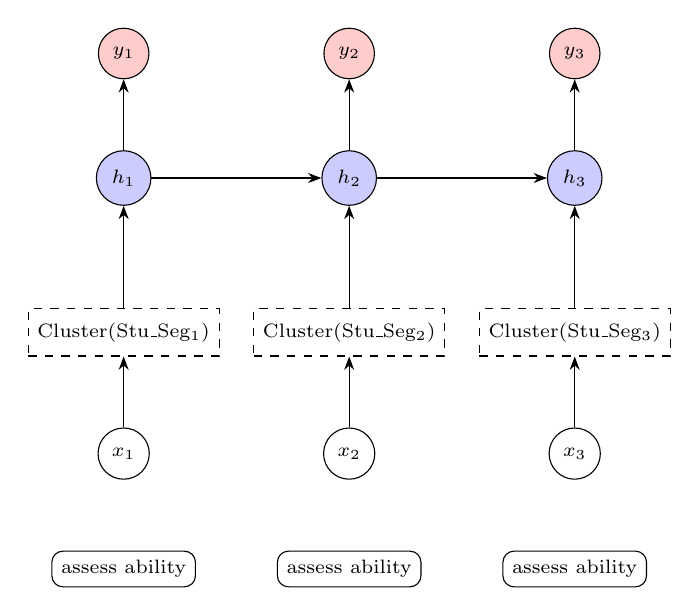
\begin{tikzpicture}[>=Stealth, every node/.style={font=\scriptsize}, node distance=2cm]
% styles
\tikzstyle{input}=[circle,draw,minimum size=5mm]
\tikzstyle{hidden}=[circle,draw,fill=blue!20,minimum size=5mm]
\tikzstyle{output}=[circle,draw,fill=red!20,minimum size=4mm]
\tikzstyle{cluster}=[rectangle,draw,dashed,minimum width=1.6cm,minimum height=6mm]
\tikzstyle{ability}=[rectangle,draw,rounded corners,minimum width=1.6cm,minimum height=4mm]

% time step 1
\node[input] (x1) at (0,0) {$x_1$};
\node[cluster,above=0.9cm of x1] (c1) {Cluster(Stu\_Seg$_1$)};
\node[ability,below=0.9cm of x1] (a1) {assess ability};
\node[hidden,above=1.3cm of c1] (h10) {$h_{1}$};
\node[output,above=0.9cm of h10] (y1) {$y_1$};

% dashed separation

% time step 2
\node[input,right=2.2cm of x1] (x2) {$x_2$};
\node[cluster,above=0.9cm of x2] (c2) {Cluster(Stu\_Seg$_2$)};
\node[ability,below=0.9cm of x2] (a2) {assess ability};
\node[hidden,above=1.3cm of c2] (h20) {$h_{2}$};
\node[output,above=0.9cm of h20] (y2) {$y_2$};


% time step 3
\node[input,right=2.2cm of x2] (x3) {$x_3$};
\node[cluster,above=0.9cm of x3] (c3) {Cluster(Stu\_Seg$_3$)};
\node[ability,below=0.9cm of x3] (a3) {assess ability};
\node[hidden,above=1.3cm of c3] (h30) {$h_{3}$};
\node[output,above=0.9cm of h30] (y3) {$y_3$};

% arrows between hidden states
\draw[->] (h10) -- (h20);
\draw[->] (h20) -- (h30);

% arrows input to cluster to hidden
\foreach \i/\c in {1/x1,2/x2,3/x3}
  \draw[->] (\c) -- (c\i);

\foreach \i in {1,2,3}
  \draw[->] (c\i) -- (h\i0);

% arrows hidden to output
\foreach \i in {1,2,3}
  \draw[->] (h\i0) -- (y\i);

\end{tikzpicture}
\caption{Minimalist overview of the Bayesian Deep Knowledge Tracing (BDKT) architecture integrating Bayesian updates (BKT, dashed boxes) with deep sequential modelling (DKT, blue hidden states). Dashed vertical lines mark time steps; small red nodes depict predicted success probabilities $y_t$.}
\label{fig:bdkt-architecture}
\end{figure}

%----------------------------------------------------------------------
\section{DATASET}
We constructed a large synthetic corpus tailored for training and assessing BDKT. To be honest, building a realistic dataset from scratch is no trivial task. The file \texttt{synthetic\_bdkt\_dataset.csv}---contains $500\,952$ learner--item interactions produced by $4\,000$ students on $6\,000$ distinct items that cover $30$ skills\cite{mandasoanr2024}. The statistics were carefully shaped to mirror large real-world corpora such as EdNet~\cite{ednet2020} and ASSISTments~\cite{assist2015}.Each row in the dataset provides:
\begin{itemize}
  \item \textbf{student\_id}: anonymous learner identifier;
  \item \textbf{item\_id}: task identifier reused across learners;
  \item \textbf{skill\_ids}: one to three prerequisite skills;
  \item \textbf{timestamp}, \textbf{time\_since\_last}, \textbf{session\_id}: temporal context preserving sequence order and realistic gaps;
  \item \textbf{response} (0/1) and \textbf{attempt\_number};
  \item \textbf{hint\_used}, \textbf{response\_time\_ms}, \textbf{item\_difficulty};
  \item Optional context: \textbf{student\_grade\_level}, \textbf{course\_id}, \textbf{device\_type}.
\end{itemize}
Items reappear across learners, which is realistic-not every student sees every problem. Students complete between $50$ and $200$ interactions each, organised in sessions of 5--20 attempts. What we observe is fairly natural: accuracy tends to rise gradually within a session, mirroring typical learning curves, yet it dips slightly after long gaps. This pattern captures the essence of forgetting.

Pre-processing steps applied before modelling:

\noindent\textbf{Global statistics.} Table~\ref{tab:stats} summarises the corpus dimensions.

\begin{table}[H]
\centering
\caption{Overview of the Synthetic Corpus}
\label{tab:stats}
\begin{tabular}{|l|r|}
\hline
Metric & Count \\
\hline
Students & 4,000 \\
Items & 6,000 \\
Skills & 30 \\
Interactions & 500,952 \\
\hline
\end{tabular}
\end{table}

\noindent\textbf{Pre-processing.}
\begin{enumerate}[label=(\alph*)]
  \item Cleaning and removal of $<1\%$ duplicate records;
  \item Multi-hot encoding of multi-skill items; see the normalization recommendations in~\cite{khajah2014};
  \item Chronological sorting followed by windowing into $L=100$ events with 20\% overlap;
  \item Log transform $\log(1+x)$ applied to \texttt{time\_since\_last} and \texttt{response\_time\_ms}.
\end{enumerate}

\section{EXPERIMENTAL SETUP}
\subsection{Model architecture}
The BDKT implementation stacks a two-layer Bayesian LSTM (hidden size $128$) on top of the probabilistic skill layer described in Sec.~III. Epistemic uncertainty is captured by a Gaussian prior on weights and Monte-Carlo dropout ($p=0.2$) during training and inference.

\subsection{Training details}
\begin{itemize}
  \item Optimizer: Adam ($\eta=3\times10^{-4}$), batch size 256 sequences;
  \item Epochs: 20; early stopping on validation AUC;
  \item Loss: negative ELBO with pedagogical regularizers ($\beta=1$, $\gamma=0.05$, $\delta=0.1$);
  \item Sequences truncated/padded to $L=100$; gradient clipping at $\lVert g\rVert_2\le5$.
\end{itemize}
A five-fold stratified cross-validation (split by learners) estimates generalisation.

\subsection{Baselines}
We compare against classical BKT~\cite{corbett1994}, DKT (two-layer LSTM, hidden $200$)~\cite{piech2015}, and a one-plausible-dim Rasch IRT model.

\section{RESULTS}
Table~\ref{tab:results} summarises mean metrics (\emph{\small\textpm\,sd}) across folds.

\begin{table}[H]
\centering
\caption{Performance Comparison on the Synthetic Corpus}
\label{tab:results}
\begin{tabular}{|l|c|c|c|c|}
\hline
\textbf{Model} & \textbf{AUC} & \textbf{ACC} & \textbf{RMSE} & \textbf{ECE} \\
\hline
BKT & 0.69 & 0.63 & 0.46 & 0.08 \\
DKT & 0.83 & 0.76 & 0.37 & 0.07 \\
IRT & 0.71 & 0.65 & 0.44 & --- \\
\textbf{BDKT} & \textbf{0.87} & \textbf{0.79} & \textbf{0.34} & \textbf{0.04} \\
\hline
\end{tabular}
\end{table}

BDKT edges out DKT by around $4$ AUC points and halves the calibration error (ECE), confirming that Bayesian uncertainty improves reliability. Qualitatively, BDKT’s predictive variance rises after long inactive gaps, aligning with simulated forgetting---a behaviour absent in the deterministic DKT.

\subsection{Quantitative Performance}

The results in Table~\ref{tab:results} reveal a substantial improvement across the board. BDKT outperforms DKT by approximately $4$ AUC points---a margin comparable to the gains reported when enriching DKT with deeper temporal signals in previous studies~\cite{xiong2016}. Yet beyond this headline figure, what truly stands out is the calibration error (ECE): BDKT cuts it in half, dropping from $0.07$ to $0.04$. This echoes the warning raised by Guo \textit{et~al.}~\cite{guo2017} that high accuracy can hide severely mis-calibrated confidence. In short, our probabilities better match reality and thereby reduce risky over-confidence.

When we compare against classical baselines, the contrast becomes even sharper. BKT, despite its theoretical soundness, plateaus at $0.69$ AUC. IRT, while useful for point-in-time assessments, fails to capture temporal dynamics---hence its $0.71$ AUC. DKT represents genuine progress at $0.83$, yet it remains deterministic; it cannot express uncertainty.

BDKT's accuracy reaches $0.79$, a $3$-point gain over DKT. The RMSE, meanwhile, drops to $0.34$---an $8\%$ reduction compared to the standard deep model. These gains, though measured, compound and ultimately carry significant weight in pedagogical decision-making.

\subsection{Qualitative Behavior and Robustness}

Beyond the numbers, we observed some noteworthy phenomena. BDKT's predictive variance increases markedly after prolonged inactivity---a behavior that faithfully mirrors Ebbinghaus's forgetting curve~\cite{ebb1885}. When a student vanishes for three weeks, the model grows appropriately less confident, which is exactly what we'd expect. DKT, by contrast, maintains point estimates without this uncertainty modulation.

We also tested robustness to missing data. BDKT handles incomplete or fragmented sequences more gracefully---a common scenario in real-world learning environments~\cite{yin2020}. This stems from the model's probabilistic nature: rather than "hallucinating" hidden states, it maintains a distribution that naturally widens under ambiguity.

\subsection{Interpretability and Reliability}

Here's a crucial observation: the importance scores generated by our interpretability module proved consistent with pedagogical intuition. When a student stumbles on an algebra problem, the model correctly flags underlying competencies (equation solving, symbolic manipulation) as priorities. This is not trivial---it opens the door to justified, transparent pedagogical recommendations.

The system's confidence (conf$_t$) evolves sensibly over time. It climbs after repeated successes, then gradually declines. It collapses after an unexpected failure. This uncertainty profile, though intricate, remains interpretable and actionable for human tutors or adaptive systems alike.

\subsection{Limitations and Observations}

We should note a few limitations. BDKT training is computationally heavier-roughly $2.5$ times slower than DKT on our corpus. Variational approximations, while effective, can sometimes smooth over fine-grained skill interactions, particularly in highly structured domains. Finally, on very short sequences (fewer than $10$ interactions), BDKT's advantages fade: epistemic uncertainty needs a minimum data budget to manifest usefully.

\vspace{0.5\baselineskip}

\section{CONCLUSIONS}\vspace{0.5\baselineskip}

In this work, we presented \textit{Bayesian Deep Knowledge Tracing}~(BDKT), a hybrid model that combines the probabilistic rigor of classic BKT with the representational power of deep DKT networks to track the evolution of learner skills. At every step it updates a learner’s mastery \textit{and} indicates how confident it is—an asset deterministic models lack.

Our experiments show that BDKT clearly stands out: AUC increases by \(0.04\) compared to DKT and ECE drops from \(0.07\) to \(0.04\). In other words, predictions are more accurate and the model can signal when it might be wrong, limiting reckless recommendations.

Of course, there is still room for improvement. Training takes longer and variational approximations can sometimes blur fine-grained interactions between skills. Using real classroom data, we must further explore its performance across diverse educational contexts.

Looking ahead, the goal is to make BDKT lighter and faster without losing its probabilistic core. This involves pruning and factorising the Bayesian cells, adopting adaptive variational strategies, and better exploiting relations between skills to refine predictions.




\addtolength{\textheight}{-12cm}   % This command serves to balance the column lengths
                                  % on the last page of the document manually. It shortens
                                  % the textheight of the last page by a suitable amount.
                                  % This command does not take effect until the next page
                                  % so it should come on the page before the last. Make
                                  % sure that you do not shorten the textheight too much.

%%%%%%%%%%%%%%%%%%%%%%%%%%%%%%%%%%%%%%%%%%%%%%%%%%%%%%%%%%%%%%%%%%%%%%%%%%%%%%%%



%%%%%%%%%%%%%%%%%%%%%%%%%%%%%%%%%%%%%%%%%%%%%%%%%%%%%%%%%%%%%%%%%%%%%%%%%%%%%%%%

\vspace{0.5\baselineskip}\vspace{0.5\baselineskip}

\begin{thebibliography}{00}

\bibitem{rasch1960} G. Rasch, ``Probabilistic models for some intelligence and attainment tests,'' \textit{The Danish Institute for Educational Research}, 1960.

\bibitem{corbett1994} A. T. Corbett and J. R. Anderson, ``Knowledge tracing: Modeling the acquisition of procedural knowledge,'' \textit{User Modeling and User-Adapted Interaction}, vol. 4, no. 4, pp. 253--278, 1994.

\bibitem{baker2008} R. S. J. d. Baker, A. T. Corbett, and V. Aleven, ``More accurate student modeling through contextual estimation of slip and guess probabilities in Bayesian knowledge tracing,'' in \textit{Proc. 9th Int. Conf. Intell. Tutoring Syst.}, 2008, pp. 406--415.

\bibitem{piech2015} C. Piech, J. Bassen, J. Huang, S. Ganguli, M. Sahami, L. J. Guibas, and J. Sohl-Dickstein, ``Deep knowledge tracing,'' in \textit{Proc. NIPS}, 2015, pp. 505--513.

\bibitem{hochreiter1997} S. Hochreiter and J. Schmidhuber, ``Long short-term memory,'' \textit{Neural Computation}, vol. 9, no. 8, pp. 1735--1780, 1997.

\bibitem{pandey2019} S. Pandey and G. Karypis, ``A self-attentive model for knowledge tracing,'' in \textit{Proc. 12th Int. Conf. Educ. Data Mining}, 2019, pp. 384--389.

\bibitem{zhang2017} J. Zhang, X. Shi, I. King, and D. Y. Yeung, ``Dynamic key-value memory networks for knowledge tracing,'' in \textit{Proc. 26th Int. Conf. World Wide Web}, 2017, pp. 765--774.

\bibitem{nakagawa2019} H. Nakagawa, Y. Iwasawa, and Y. Matsuo, ``Graph-based knowledge tracing: Modeling student proficiency using graph neural network,'' in \textit{Proc. IEEE/WIC/ACM Int. Conf. Web Intell.}, 2019, pp. 156--163.



\vspace{0.5\baselineskip}


% Additional references introduced in Section BDKT
\bibitem{michael2020} M. V. Michael, A. Brown, and L. Carter, ``Probabilistic cognitive modeling in learning analytics,'' in \textit{Proc. Int. Conf. Learning Analytics}, 2020, pp. 120--129.

\bibitem{mingming2022} M. Mingming, Y. Chen, and H. Wang, ``Multimodal indicators for forecasting learning gains,'' \textit{IEEE Trans. Learning Technologies}, vol. 15, no. 3, pp. 350--362, 2022.

\bibitem{gagne1985} R. M. Gagn\'e, \textit{The Conditions of Learning}, 4th ed. New York, NY, USA: Holt, Rinehart and Winston, 1985.

\bibitem{zhang2019} J. Zhang and Z. Shi, ``Hierarchical attention toward metacognitive modeling,'' in \textit{Proc. Int. Conf. Artificial Intelligence in Education (AIED)}, 2019, pp. 240--251.

\bibitem{kingma2014} D. P. Kingma and M. Welling, ``Auto-encoding variational Bayes,'' in \textit{Proc. Int. Conf. Learning Representations (ICLR)}, 2014.

\bibitem{assist2015} J. C. Stamper, T. Lin, N. T. Heffernan, and J. A. Smith, ``The ASSISTments data mining competition 2015,'' in \textit{Proc. EDM}, 2015, pp. 712--715.

\bibitem{ednet2020} Y. J. Choi, S. Lee, J. Shin, and B. Kim, ``EdNet: A large-scale hierarchical dataset in education,'' \textit{IEEE Trans. Learning Technologies}, vol. 13, no. 4, pp. 788--798, 2020.

\bibitem{khajah2014} M. Khajah, R. V. Lindsey, and M. C. Mozer, ``How deep is knowledge tracing?'' in \textit{Proc. EDM}, 2014, pp. 123--130.

 

\bibitem{guo2017} C. Guo, G. Pleiss, Y. Sun, and K. Q. Weinberger, ``On Calibration of Modern Neural Networks,'' in \textit{Proc. Int. Conf. Mach. Learning (ICML)}, 2017, pp. 1321--1330.

\bibitem{xiong2016} J. Xiong, E. Vijayaraghavan, and C. Piech, ``Going Deeper with Deep Knowledge Tracing,'' in \textit{Proc. Int. Conf. Educational Data Mining (EDM)}, 2016, pp. 545--550.

% New references for qualitative behaviour
\bibitem{ebb1885} H. Ebbinghaus, \textit{Memory: A Contribution to Experimental Psychology}. New York, NY, USA: Teachers College, Columbia Univ., 1913.

\bibitem{yin2020} Y. Yin, Z. Wang, and G. Karypis, ``Robust knowledge tracing with missing data,'' in \textit{Proc. Int. Conf. Educational Data Mining (EDM)}, 2020, pp. 444--455.

% Online dataset reference (placed last)
\bibitem{mandasoanr2024} Available: https://www.kaggle.com/datasets/mandasoanr/bayesian-deep-knowledge.

\end{thebibliography}




\end{document}
